\documentclass[12pt]{article}
\usepackage[margin=1 in]{geometry}
\usepackage{graphicx}
\usepackage{float}
\usepackage{booktabs}
\usepackage{siunitx}
\usepackage{amsmath}
\usepackage{amssymb}

\title{Lab 11: Op-Amp Circuits, Design and Limitations}
\author{Sean Balbale}
\date{November 19th, 2024}
\setlength{\parindent}{0in}

\begin{document}

\begin{titlepage}
  \begin{center}
    \vspace*{1in}

    \Huge
    \textbf{Lab 11}

    \LARGE
    Op-Amp Circuits, Design and Limitations

    \vspace{3 in}

    \textbf{Student Name:} Sean Balbale
    \\ \textbf{Instructor:} Dr. Iman Salama
    \\ \textbf{Lab Partner Name:} Krish Gupta
    \\ \textbf{Date:} November 19, 2024

    \vfill

  \end{center}
\end{titlepage}

\newpage

\section{Introduction}

\section{Results}
% \begin{figure}[H]
%   \centering
%   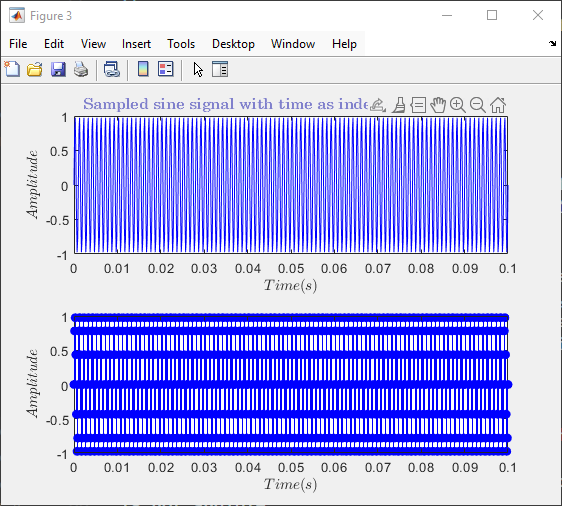
\includegraphics[width=0.3\textwidth]{fig 1f 7000.png}\hfill
%   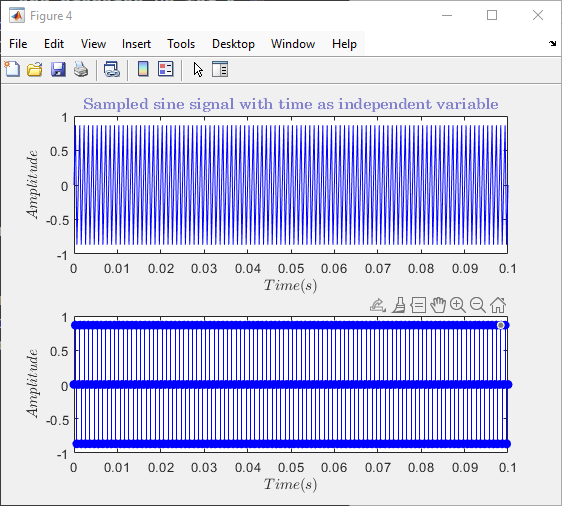
\includegraphics[width=0.3\textwidth]{fig 1f 3000.png}\hfill
%   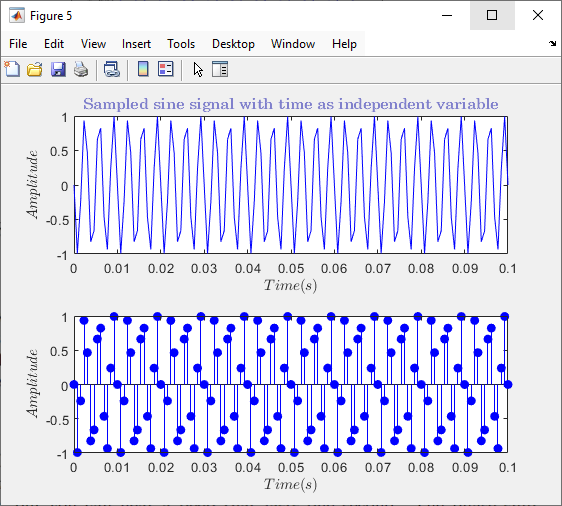
\includegraphics[width=0.3\textwidth]{fig 1f 1300.png}
%   \caption{Sinusoidal with $f_s$ = 7 kHz, 3 kHz, and 1.3 kHz}
%   \label{fig:fig3}
% % \end{figure}


\section{Discussion and Conclusion}


\section{References}
[1] Dr. Iman Salama. “Lab 11 – Op-Amp Circuits, Design and Limitations” Northeastern University. 11 November 2024.

\end{document}
